\section{Cpp\-Logger Class Reference}
\label{classCppLogger}\index{CppLogger@{CppLogger}}
{\tt \#include $<$Cpp\-Logger.hpp$>$}

Inheritance diagram for Cpp\-Logger::\begin{figure}[H]
\begin{center}
\leavevmode
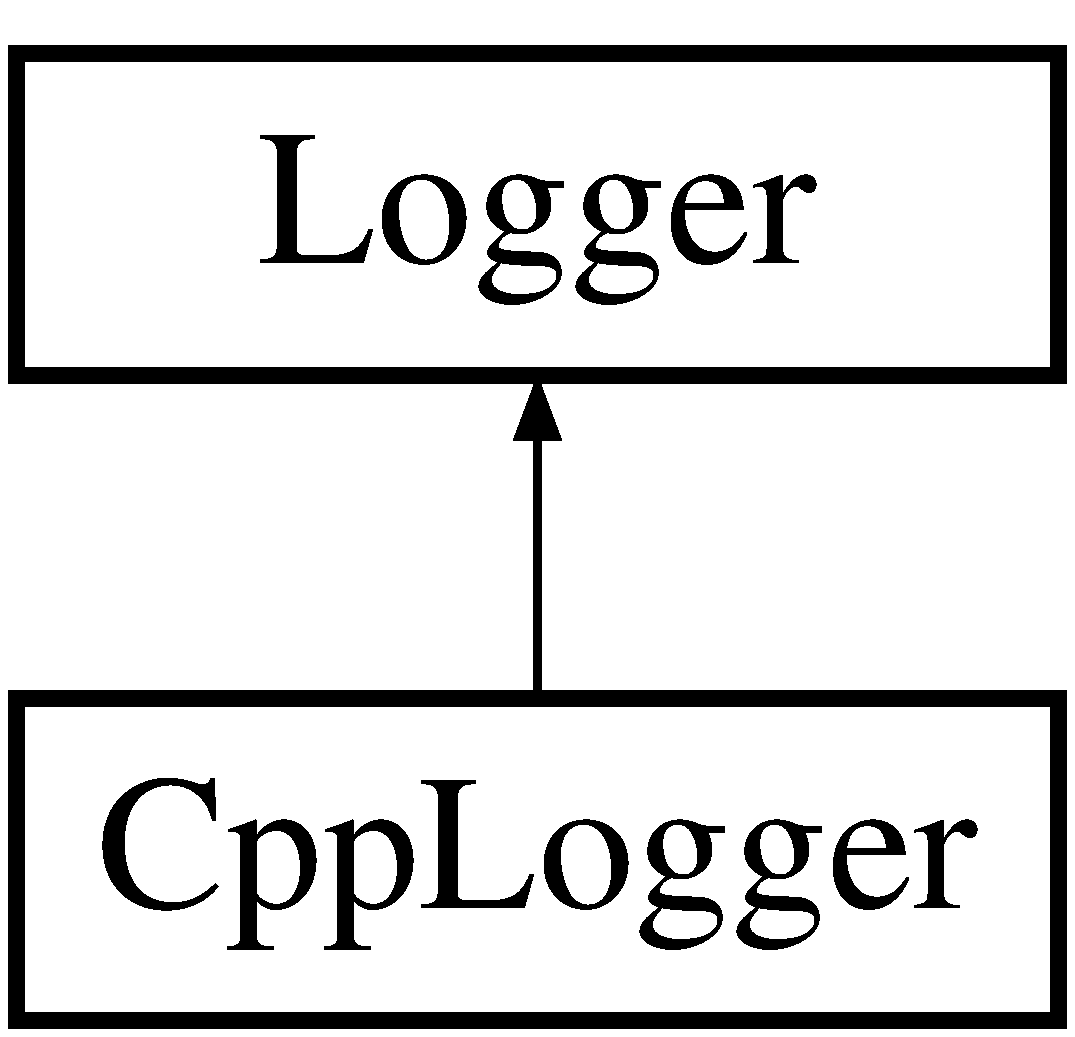
\includegraphics[height=2cm]{classCppLogger}
\end{center}
\end{figure}
\subsection*{Public Member Functions}
\begin{CompactItemize}
\item 
{\bf Cpp\-Logger} (const {\bf Cpp\-Logger} \&rhs)
\item 
{\bf Cpp\-Logger} (ostream \&log=cerr, int n\-Log\-Level=0)\label{classCppLogger_a1}

\item 
virtual {\bf $\sim$Cpp\-Logger} ()
\item 
virtual void {\bf log} (int level=ERROR\_\-MESSAGES\_\-LR, const std::string \&message=\char`\"{}\char`\"{}) const 
\end{CompactItemize}


\subsection{Detailed Description}
Provides a ofstream interface to the {\bf Logger}{\rm (p.\,\pageref{classLogger})} system.



\subsection{Constructor \& Destructor Documentation}
\index{CppLogger@{Cpp\-Logger}!CppLogger@{CppLogger}}
\index{CppLogger@{CppLogger}!CppLogger@{Cpp\-Logger}}
\subsubsection{\setlength{\rightskip}{0pt plus 5cm}Cpp\-Logger::Cpp\-Logger (const {\bf Cpp\-Logger} \& {\em rhs})\hspace{0.3cm}{\tt  [inline]}}\label{classCppLogger_a0}


Description: Copies an existing logger.\index{CppLogger@{Cpp\-Logger}!~CppLogger@{$\sim$CppLogger}}
\index{~CppLogger@{$\sim$CppLogger}!CppLogger@{Cpp\-Logger}}
\subsubsection{\setlength{\rightskip}{0pt plus 5cm}virtual Cpp\-Logger::$\sim$Cpp\-Logger ()\hspace{0.3cm}{\tt  [inline, virtual]}}\label{classCppLogger_a2}


Description: Currently does nothing since the {\bf Logger}{\rm (p.\,\pageref{classLogger})} does not allocate resources to itself.

\subsection{Member Function Documentation}
\index{CppLogger@{Cpp\-Logger}!log@{log}}
\index{log@{log}!CppLogger@{Cpp\-Logger}}
\subsubsection{\setlength{\rightskip}{0pt plus 5cm}virtual void Cpp\-Logger::log (int {\em level} = {\tt ERROR\_\-MESSAGES\_\-LR}, const std::string \& {\em message} = {\tt \char`\"{}\char`\"{}}) const\hspace{0.3cm}{\tt  [virtual]}}\label{classCppLogger_a3}


Description: Tests the log level of the message and reports the message if it has a high enough priority otherwise the message is suppressed.

The documentation for this class was generated from the following file:\begin{CompactItemize}
\item 
Cpp\-Logger.hpp\end{CompactItemize}
